\section{Single Variable Statistics}
    
    \subsection{Intro to Statistics}
    This is a massive shift compared to the rest of the stuff we've done so far. It is a lot of (relatively simple) graphing, and data management, and also includes a lot of spreadsheet work (which I may or may not include). Using a frequency table will help you, as well as attention to detail.
    
    \subsection{Displaying Frequency}
    To start, we're going to have to (re)define some stuff you have learned in earlier years. This will seem like a lot at first, but most of it is quite basic, and there are no equations to memorize.
    \begin{definition}
        Range: A range, in relation to sets of data, is how far apart the data points are spread. It is calculated by taking the largest number, and subtracting it by the smallest. 
    \end{definition}
    \begin{definition}
        Frequency Diagram: A frequency diagram is a graph used to show the frequency of various points, or intervals of data (ex. years, or decades). 
    \end{definition}
    \begin{definition}
        Frequency Polygon: A shape that helps the reader understand the overall shape of the diagram or distribution.
    \end{definition}
    \begin{center}
        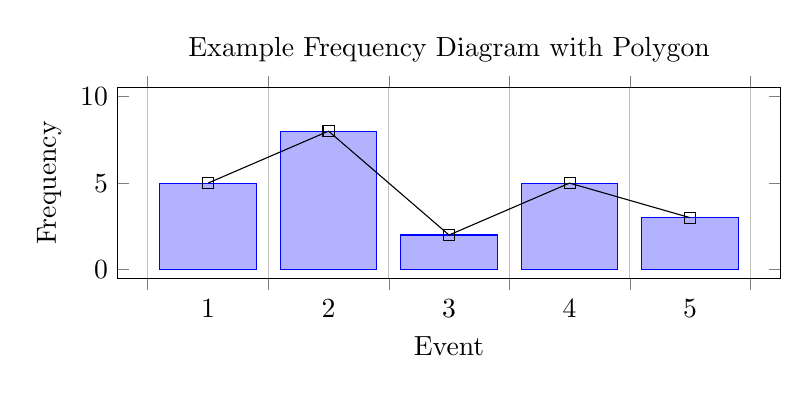
\begin{tikzpicture}
            \begin{axis}[
                width=10cm,
                height=4cm,
                x tick label style={
                	/pgf/number format/1000 sep=},
                title=Example Frequency Diagram with Polygon,
                ylabel=Frequency,
                xlabel=Event,
                ymin=0,
                ymax=10,
                xmin=1,
                xmax=6,
                enlargelimits=0.05,
                ybar interval=0.8,
            ]
            \addplot
                coordinates {
                    (1,5)
                    (2,8)
                	(3,2)
                	(4,5)
                	(5,3)
                	(6,0.0000)};
            \addplot[sharp plot,mark=square]
                coordinates {
                    (1.5,5)
                    (2.5,8)
                	(3.5,2)
                	(4.5,5)
                	(5.5,3)};
            \end{axis}
        \end{tikzpicture}
    \end{center}
    \begin{definition}
        Cumulative Frequency: This refers to the running total of frequencies. Shown below is an example of once such diagram.
    \end{definition}
    \begin{center}
        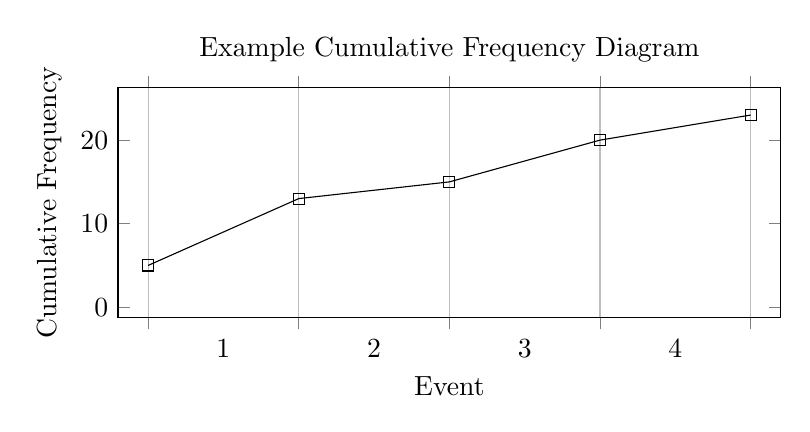
\begin{tikzpicture}
            \begin{axis}[
                width=10cm,
                height=4.5cm,
                x tick label style={
                	/pgf/number format/1000 sep=},
                title=Example Cumulative Frequency Diagram,
                ylabel=Cumulative Frequency,
                xlabel=Event,
                ymin=0,
                ymax=25,
                xmin=1,
                xmax=5,
                enlargelimits=0.05,
                ybar interval=1,
            ]
            \addplot[sharp plot,mark=square]
                coordinates {
                    (1,5)
                    (2,13)
                	(3,15)
                	(4,20)
                	(5,23)
                };
            \end{axis}
        \end{tikzpicture}
    \end{center}
    \begin{definition}
        Relative Frequency: This means the frequency expressed as a percentage, found by dividing the frequency by the total number of results.
    \end{definition}
    \begin{center}
        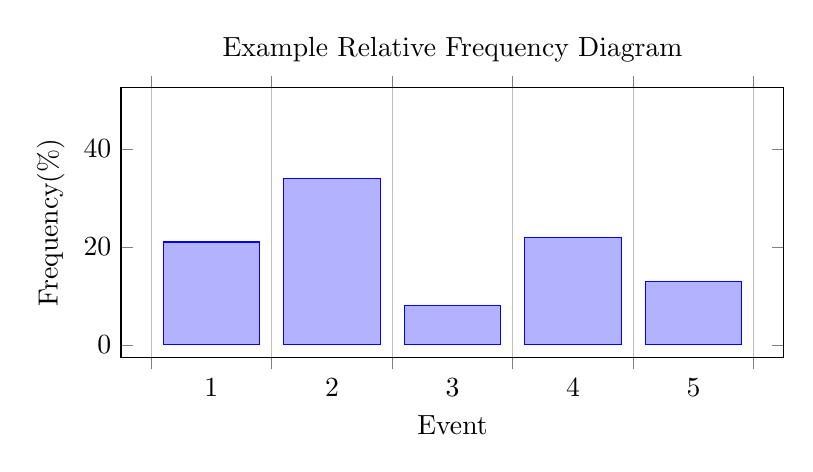
\begin{tikzpicture}
            \begin{axis}[
                width=10cm,
                height=5cm,
                x tick label style={
                	/pgf/number format/1000 sep=},
                title=Example Relative Frequency Diagram,
                ylabel=Frequency(\%),
                xlabel=Event,
                ymin=0,
                ymax=50,
                xmin=1,
                xmax=6,
                enlargelimits=0.05,
                ybar interval=0.8,
            ]
            \addplot
                coordinates {
                    (1,21)
                    (2,34)
                	(3,8)
                	(4,22)
                	(5,13)
                	(6,0.0000)};
            \end{axis}
        \end{tikzpicture}
    \end{center}
    \begin{definition}
        Histogram: Essentially a bar graph, yet with the data in groupings, instead of being separate.
    \end{definition}
    \begin{center}
        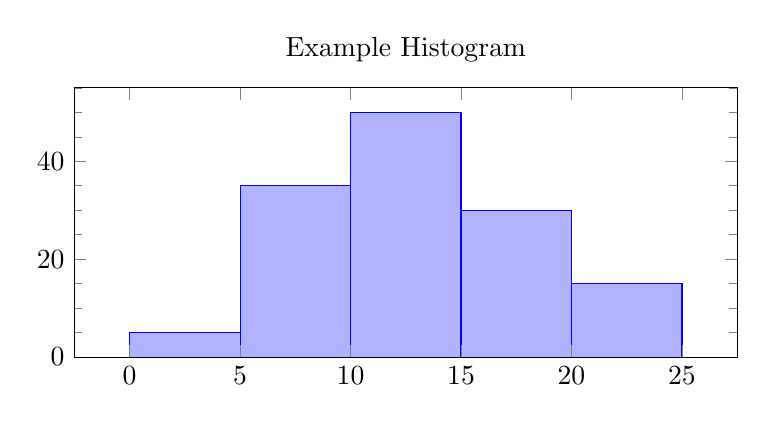
\begin{tikzpicture}
            \begin{axis}[
                x tick label style={
                	/pgf/number format/1000 sep=},
                title=Example Histogram,
                width=10cm,
                height=5cm,
                ymin=0,
                ymax=55,
                minor y tick num = 3,
                area style,
            ]
            \addplot+[ybar interval,mark=no] plot coordinates {
                (0, 5)
                (5, 35)
                (10, 50)
                (15, 30)
                (20, 15)
                (25, 0)};
            \end{axis}
        \end{tikzpicture}
    \end{center}
    All of this data and results above can be displayed and organized in something called a frequency table, as defined, and shown below.
    \begin{definition}
        Frequency Table: This is a table that contains all of the above results, as well as tallies of data points.
    \end{definition}
    \begin{center}
        \begin{tabular}{ | l | l | l | l |}
            \hline
            (x) & Frequency & Relative Frequency & Cumulative Frequency \\ \hline
            1 & 5 & $\frac{5}{23}$=21\% & 5 \\ \hline
            2 & 8 & $\frac{8}{23}$=34\% & 13 \\ \hline
            3 & 2 & $\frac{2}{23}$=8\% & 15 \\ \hline
            4 & 5 & $\frac{5}{23}$=22\% & 20 \\ \hline
            5 & 3 & $\frac{3}{23}$=13\% & 23 \\ \hline
        \end{tabular}
    \end{center}
    
    \subsection{Measures of Central Tendency}
    Measures of Central Tendency deal with the various numbers we use to find data points we can make assumptions based on.
    These three numbers we use are called the \textbf{mean, median and mode}.
    \begin{definition}
        Mean: The mean represents the average of the data, and is found by using the equation below.
        \begin{equation*}
            \mean{x} = \frac{\sum x}{n}
        \end{equation*}
    \end{definition}
    \begin{definition}
        Median: The median represents the middle-most point of data, for example in a set of 5 integers, the median will be the third.
        To find the median of an list of data of which \textbf{n is odd numbered} you can use the equation below.
        \begin{equation*}
            \median{x} = \mbox{\emph{Number in middle of data}}
        \end{equation*}
        if the equation is even numbered, you must use the average of the numbers that the median is in between.
        For example if you have a list of 8 numbers, the median would be the average of 4 and 5.
        The equation for this can be seen below.
        \begin{equation*}
            \median{x} = \frac{\mbox{\emph{Left Number + Right Number}}}{2}
        \end{equation*}
    \end{definition}
    \begin{definition}
        Mode: The mode represents the data point that has been repeated the most often. Can be found by merely looking at the highest repeated data set.    
    \end{definition}
    
    \subsection{Measures of Spread}
    A measure of spread is a measurement that describes how the data is distributed, and how widely it fluctuates.
    To measure these, we divided the spread of the data into something called \emph{quartiles.}
    A quartile, just like its name implies, is merely a quarter of the data.
    The first Quartile (referred to henceforth as Q1) is the median of the \textbf{FIRST HALF} of the data, Q2 is the middle (or median), and Q3 is the median of the \textbf{LAST HALF} of the data.
    If we want to find the most relevant data, we'll typically look at the data between Q1 and Q3, this range of data is called the Inter Quartile Range (IQR).
    \begin{definition}
        Inter Quartile Range: This is the middle-most data, and a grouping you can easily make assumptions from. To find this, we use the equation below.
        \begin{equation*}
            \mbox{IQR} = \mbox{Q3}-\mbox{Q1}
        \end{equation*}
    \end{definition}
    Using this, we can also find other data to make assumptions off of, such as the Semi-Inter Quartile Range.
    \begin{definition}
        Semi Inter Quartile Range: This is $\frac{1}{2}$ of the difference of the IQR, and therefore is less affected by outliers. Can also be referred to as the SIQR, and is found by the equation below.
        \begin{equation*}
            \mbox{SIQR} = \frac{\mbox{IQR}}{2}
        \end{equation*}
    \end{definition}
    We can display these using something called a \textbf{box and whisker plot}.
    This will show Q1, Q2, and Q3, along with the highest and lowest datum.
    An example of this is shown below.
    \begin{center}
        \begin{tikzpicture} [thick, framed]
            \filldraw[fill=green!20] (2.85,0) rectangle (5.7,1);
            \draw (4.45,0)--(4.45,1) node[above]{$\textsc{M}$};
            \draw (5.7,0.5)--(11,0.5);%vandret linie til max
            \draw (2.85,0.5)--(1,0.5);%vandret linie til min
            \draw (11,0.39)--(11,0.61);
            \draw (1,0.39)--(1,0.61);
            \draw [
                postaction={
                    draw,
                    decoration=ticks,
                    segment length=1cm,
                    decorate,
                }
             ] (0,-1) -- (11,-1);
             \foreach \tick in {0,...,11}
                \node at (\tick,-1) [below=1pt] {\tick};
        \end{tikzpicture}
    \end{center}
    \subsection{Intro to Variance}
    To calculate the variance, we must first calculate the deviations. 
    A deviation is the difference between an individual value in a data set and the mean of that set.
    To calculate the deviation, we'll need to use the equation below.
    \begin{equation*}
        \mbox{Deviation}= x - \mean{x}
    \end{equation*}
    We use different kinds of deviations for various reasons, such as Mean Deviations ($md$) and Standard Deviations ($\sigma$) They are defined below, though most typically we will use the Standard Deviation. Most of these can be calculated much easier if you use the \emph{STAT} mode on your calculator, but the equations will be below if your calculator doesn't support that.
    \begin{definition}
        Mean Deviation: The mean deviation is the mean of all the distances to the mean. To calculate this, we'll use the formula below to solve for $md$, which represents the mean deviation. 
        \begin{equation*}
            md = \frac{\sum|x-\mean{x}|}{n}
        \end{equation*}
    \end{definition}
    \begin{definition}
        Standard Deviation: This is more widely used, and differs from the mean deviation in the fact that it uses square roots and exponents rather than the absolute value function. Will always be bigger than the mean deviation, and is shown as $(\sigma)$. 
        \begin{equation*}
            \sigma = \sqrt{\frac{\sum(x-\mean{x})^2}{n}}
        \end{equation*}
    \end{definition}
    Once we know the deviation, we can find the variance of various numbers.
    \begin{definition}
        Variance: This number represents the average of the squares of the deviations. You can find this by simply squaring the Standard Deviation (giving you $\sigma^{2}$), or by using the equation below.
        \begin{equation*}
            Variance = \frac{\sum(x-\mean{x})^{2}}{n}
        \end{equation*}
    \end{definition}
    
    \subsection{Z\textemdash Scores}
    A Z-Score is the number of Standard Deviations that a datum is from the mean. We can find this using the equation below. 
    \begin{equation*}
        z = \frac{x-\mean{x}}{\sigma}
    \end{equation*}
    If $z<0$ the element is less than the mean, if $z=0$, the element is equal to the mean, and if $z>0$, the number is greater than the mean.
    
    \subsection{Deviations with Intervals Data}
    When data is grouped into intervals, the formula for mean deviation and standard deviation change. Mean Deviation changes to the equation below.
    \begin{equation*}
        md = \frac{\sum f|x-\mean{x}|}{n}
    \end{equation*}
    Standard Deviation also changes into the formula below.
    \begin{equation*}
        \sigma = \sqrt{\frac{\sum f(x-\mean{x})^2}{n}}
    \end{equation*}
    In both of these equations, $f$ represents the frequency of the interval. 
    
    \subsection{Chebyshev's Theorem}
    Chebyshev's Theorem states that given a set of data with a mean (designated $\mean{x}$) and a Standard Deviation ($\sigma$), then \textbf{at least} x\% of the will be within $k$ standard deviations of the mean. We find this using the equation below.
    \begin{equation*}
        x = (1-\frac{1}{k^2})\%
    \end{equation*}
    
    \subsection{Gathering Data}
    This subsection is entirely definitions, and as such is quite lengthy. It is tested on, but I believe it is multiple choice. As such this is semi-important if any research or actual studies are ever done in your class, or in the real world. 
    \begin{definition}
        Population: Refers to individuals who belong to a group being studied. 
    \end{definition}
    \begin{definition}
        Sample: A subset of a population
    \end{definition}
    \begin{definition}
        Simple Random Sample: Every member of the population has an equal chance of being selected.  
    \end{definition}
    \begin{definition}
        Systematic Sample: Selected by iterating through the population and selecting members at regular intervals.   
    \end{definition}
    \begin{definition}
        Stratified Sample: A group of population members with similar characteristics is called a stratum. A stratified sample has the same proportion of members from each stratum. 
    \end{definition}
    \begin{definition}
        Cluster Sample: When certain groups are representative of the entire population, this takes a random selection of such groups. 
    \end{definition}
    \begin{definition}
        Multistage Sample: Uses several levels of random sampling, randomly sample from groups within groups. 
    \end{definition}
    \begin{definition}
        Voluntary Response Sample: Researcher invites any member of population to participate. Results skewed as people who choose to participate not always representative of the population.
    \end{definition}
    \begin{definition}
        Convenience Sample: Easily accessible sample of the population.
    \end{definition}
    \begin{definition}
        Bias: Any factor that favors certain outcomes or responses
    \end{definition}
    \begin{definition}
        Sampling Bias: Occurs when the sampling frame does not reflect the characteristics of the population.
    \end{definition}
    \begin{definition}
        Non-response Bias: Occurs when particular groups are under-represented because they choose to not participate.   
    \end{definition}
    \begin{definition}
        Measurement Bias: Occurs when the data collection method consistently misrepresents the characteristics of a population.    
    \end{definition}
    \begin{definition}
        Response Bias: Occurs when the participants in a survey deliberately give false/misleading answers.
    \end{definition}